\documentclass[sigconf]{acmart}
% Cleaning
\usepackage{pifont}
\pagestyle{fancy} % removes running headers
\settopmatter{printacmref=false} % Removes citation information below abstract
\renewcommand\footnotetextcopyrightpermission[1]{} % removes footnote with conference information in first column
\pagestyle{plain} % removes running headers
\fancyhead{}
\settopmatter{printacmref=false, printfolios=false}
% Copyright
\setcopyright{none}
% \setcopyright{acmcopyright}
% \setcopyright{acmlicensed}
% \setcopyright{rightsretained}
% \setcopyright{usgov}
% \setcopyright{usgovmixed}
% \setcopyright{cagov}
% \setcopyright{cagovmixed}
\settopmatter{printacmref=false} % Removes citation information below abstract
\acmDOI{}


\setlength{\parskip}{0pt}
\setlength{\parsep}{0pt}
\setlength{\headsep}{0pt}
\setlength{\topskip}{0pt}
\setlength{\topmargin}{0pt}
\setlength{\topsep}{0pt}
\setlength{\partopsep}{0pt}
%\linespread{0.95}
\usepackage{mdwlist}
\usepackage{amsmath}

\usepackage{xcolor}
\newcommand{\todo}[1]{{\color{red}[TODO: #1]}}

\begin{document}
\title{TRIAD: Trusted RDF Interoperable Agent Data -- Background and Related Work}

\author{Asish A. George}
\affiliation{
  \institution{University of Victoria, Canada}
}
\email{asishgeorge@uvic.ca}

\author{Mohamed Khaled}
\affiliation{
  \institution{University of Victoria, Canada}
}
\email{mabuela@uvic.ca}

% ABSTRACT: written last (Khaled).
\begin{abstract}
\todo{Abstract, written last.}
\end{abstract}
\keywords{Data Models, FHIR, Provenance, Clinical Records, Agent Memory}
\maketitle

% INTRODUCTION: Khaled.
\section{Introduction}
\todo{Introduction.}

% HISTORY: Asish.
\subsection{History}
\todo{History (Asish).}

\section{Prior Work}
\begin{figure}
    \centering
    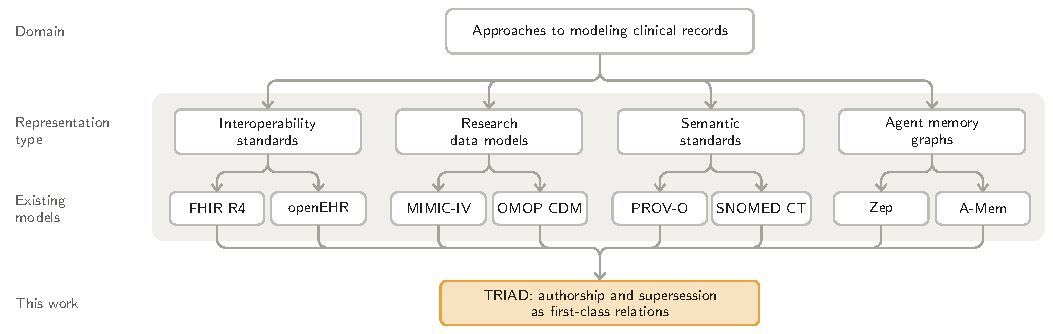
\includegraphics[width=\columnwidth]{figures/taxonomy.pdf}
    \caption{Categories of data representations relevant to clinical records.}
    \label{fig:taxonomy}
\end{figure}

% COMPARATIVE ANALYSIS: Asish (FHIR, clinical systems) + Khaled (research models).
\subsection{Comparative Analysis}
\todo{Comparison table and prose.}

% POSITIONING (Section 2.5 of the manual): Khaled's text, AI-edited for clarity (Level C). Original in appendix.
\section{Positioning and Draft ER Diagram}

In clinical settings, information moves through many hands: from the patient to the medical office assistant (MOA), then to the nurse, and finally to the physician. This movement introduces two problems. First, clinical information originates as unstructured natural language, and detail is lost each time it is transferred and recorded. Second, because a patient returns repeatedly and revises or adds to earlier accounts, records accumulate inconsistencies over time: most new facts are really updates to older ones, yet they are stored as independent entries, leaving contradictions unresolved. Underlying both is a lack of accountability and traceability. Existing models record authorship and revision only optionally, or per document rather than per fact, so a physician inheriting the record cannot reliably tell the nurse's addition from the assistant's omission, nor the current fact from a superseded one.

TRIAD addresses these gaps with two structural additions. First, authorship is attached to every individual fact: each fact records who asserted it and in what role, so the patient's own account, the assistant's intake note, the nurse's recommendation, and the physician's decision remain distinct and are never conflated. Second, revision is made explicit through typed supersession links: when a fact changes, the model preserves both the earlier version and the one that replaced it, recording what superseded what. Together these restore accountability and traceability, since every fact is attributable and every change is recoverable, and they resolve inconsistency directly: the current fact is the one with nothing superseding it, retrievable in a single step rather than reconstructed by comparing dates across scattered entries.

Structurally, both additions are carried by a central \textit{Assertion} entity, shaded grey in Figure~\ref{fig:erd}. Each Assertion links through three binary relationships: to the \textit{Staff} member who made it, through \textit{Asserts}; to the \textit{ClinicalFact} it concerns, through \textit{About}; and to the \textit{Message} it was extracted from, through \textit{ExtractedFrom}. These capture who asserted what, and from which source, giving each fact full authorship and traceability back to its origin. Revision is captured by the unary \textit{Supersedes} relationship on Assertion, with the roles \textit{Replaces} and \textit{ReplacedBy}, so the current version and its history are both preserved. The full diagram is available in our repository.

\bibliographystyle{ACM-Reference-Format}
\bibliography{bibliography.bib}

\newpage
\begin{figure*}[p]
    \centering
    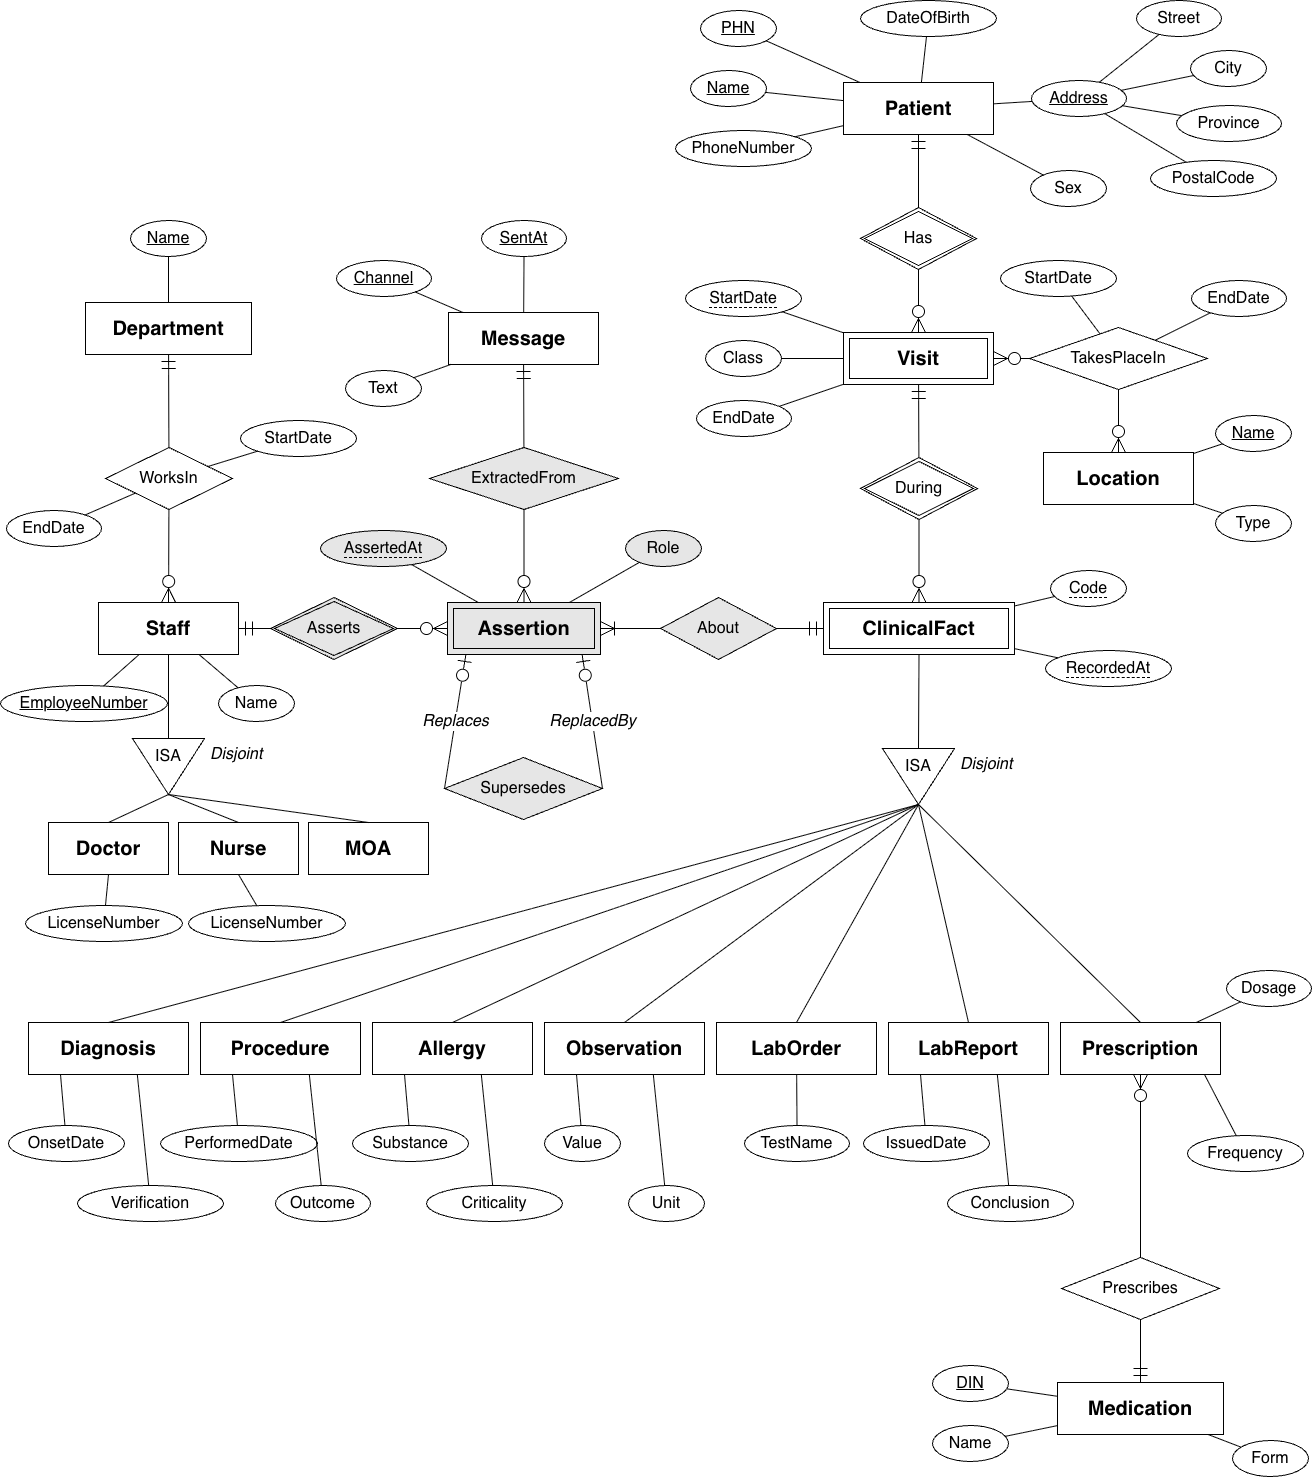
\includegraphics[width=\textwidth,height=0.93\textheight,keepaspectratio]{figures/TRIAD_ERD.png}
    \caption{The draft version of TRIAD's conceptual ER diagram. Grey marks TRIAD's contribution: who asserted each fact and in what role (Asserts), the fact asserted (About), revision (Supersedes), and the message each assertion was extracted from (ExtractedFrom). White entities align with FHIR R4. Double boxes are weak entities; a solid underline marks a key and a dashed underline a partial key. Both IS-A hierarchies are disjoint. The draw.io source is in the repository (github.com/MohamedKhalidmk/TRIAD).}
    \label{fig:erd}
\end{figure*}

% ---------------------------------------------------------------
% APPENDIX: original text before AI-assisted editing (Level C).
% Does not count toward the page limit.
% ---------------------------------------------------------------
\clearpage
\appendix
\section{Original Work Before AI-Assisted Editing}
Per the Level C guideline, this appendix contains the authors' original text, written without AI, before AI-assisted editing. AI (Claude) was also used to locate and explain sources and to render the ER diagram from the authors' design.

\subsection{Positioning: The Gap}
\textit{Spoken draft by Mohamed Khaled, with filler words removed.}

The gap is that medical data moves between different people: from the patient himself, to the MOA, then to the nurse, and finally it reaches the doctor. This movement of information has two problems. First, this information is mostly natural language, and when it gets assigned to a database, more information can get lost between the transfers. Second, we have inconsistencies over time, especially knowing that the patient can come multiple times and can change his words or add things. We end up with all this information about a patient, and most of it is just updates of the old information, but we don't know that, we just add it, so we have inconsistencies over time. There is also no accountability: if the MOA missed something or the nurse added something, we don't know whether it was the nurse's addition or the MOA's omission. We have no accountability and no traceability.

\subsection{Positioning: What TRIAD Adds}
\textit{Spoken draft by Mohamed Khaled, with filler words removed.}

It has two things. First, authorship on each and every fact: this fact was said by the patient himself, this fact was added by the MOA, this fact was added by the nurse, this fact was removed by the doctor. We have authorship on every single fact. For example, the nurse can add things, and we want to know this is the nurse's recommendation; we don't want it mixed with what the patient actually said. Hand in hand with that comes supersession: we have who changed what and who did what. We keep the old version, so when a fact changes, we have the old one and the changed fact. That gives us traceability of what could get lost, and it removes contradictions, because the current fact is a new one we can pull faster, and we still have the backup.

\subsection{Positioning: The Structure}
\textit{Spoken draft by Mohamed Khaled, with filler words removed.}

We have a main entity, the Assertion. This Assertion has three binary relationships, with the Message, the Staff, and the ClinicalFact, because we want to know who asserted it (Staff), what specific fact was asserted (ClinicalFact), and from what message. So we have full authorship and full traceability. This entity also has a unary relationship, Supersedes, which records what got replaced by what.

\end{document}
